% -*- root: ../../DAT2-A423_Project_Report.tex -*-
\section{LSB implementation}
\label{sec:lsb-implementation}
During the beginning of the project, to learn more and understand how this algorithm works, as well as see first-hand what social media sites re-encoded images, we created a small prototype of a programme, which is able to conceal an image within another image, using the LSB algorithm. 

By storing the information we want concealed in the two least significant bits, we can keep a lot of the original information, and by only each pixel of the vessel image, by a maximum value of 3 or $00000011_2$, the concealed image will almost be invisible to the naked eye.

To do this, we had to make some restrictions on how big the vessel image had to be relatively to the to-be-concealed image. To not cause corruption and to ensure all information got saved, the vessel image has to be four times as big as the hidden image, more specifically twice its height, and twice its width. Each pixel of the concealed image will be stored within four pixels of the vessel image, each masked differently, hence the vessel image has to be four times its size. We do this to get as much of the concealed image's information stored within the vessel as possible.

To make both images easier to work with, we store each pixel's colour in their own Color array. To store each pixel within the vessel, we first mask the vessel to remove the information stored within the least significant bits using the bitwise operator \&. We then mask the concealed image to only keep the information stored in two bits, then right-shift those bits so the result, will be a byte where only the least-significant-bits, can be 1, and then, add this information to the vessel. The result will be a slightly changed pixel by a value between 0 and 3 for the Red, Green and Blue channels. The first pixel in the vessel will contain the two most significant bits of the concealed image, the next will contain the third and fourth, and so on. To get back the image information, we once again use the bitwise \& operator, to only keep the information within the least-significant bits of every pixel, then left-shift them accordingly and save this to a Color array. Once every pixel has been read, the Color array can be transformed into an image which looks just like the original.

The result of concealing \ref{img2}, within \ref{img1}, can be seen in \ref{img3}

\begin{figure}[]
	\centering
	\begin{subfigure}[b]{.3\linewidth}
		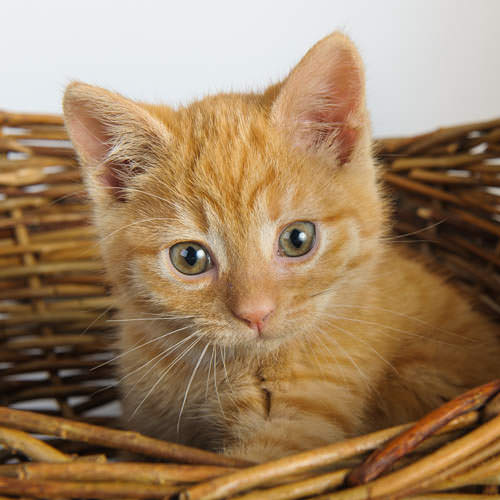
\includegraphics[width=\linewidth]{sections/pictures/vessel.jpg}
		\captionof{figure}{Vessel image}
		\label{img1}
	\end{subfigure}
	\hspace{.02\linewidth}
	\begin{subfigure}[b]{.3\linewidth}
		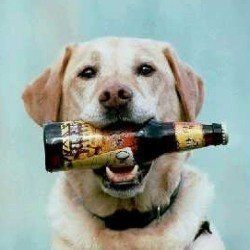
\includegraphics[width=\linewidth]{sections/pictures/concealed.jpg}
		\captionof{figure}{Concealed image}
		\label{img2}
	\end{subfigure}
	\hspace{.02\linewidth}

	\begin{subfigure}[b]{.4\linewidth}
		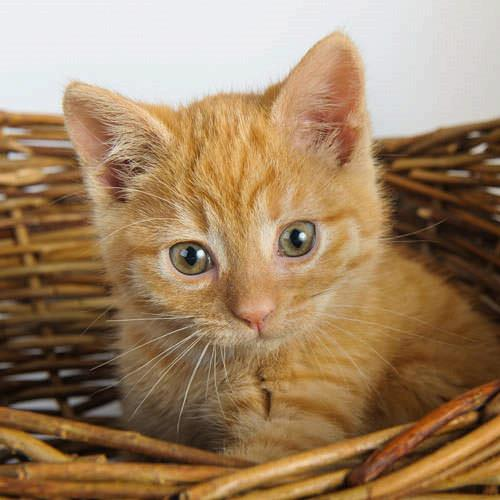
\includegraphics[width=.97\textwidth]{sections/pictures/encrypted.jpg}
		\captionof{figure}{Steganographic image}
		\label{img3}
	\end{subfigure}
	\caption{The steganographic process}\label{LSBDemo}
\end{figure} 
